The scope of this work includes development and demonstration of
various methods and tools to leverage Cyclus' existing
capabilities to model real-world fuel cycle transition scenarios.

\section{Background and motivation}
Increasing climate change concerns have directed attention
to nuclear energy, which produces reliable base load energy
with negligible CO$_2$ emission. To reduce CO$_2$ emissions,
the world will have to reduce fossil fuel based power plants.
Also, the energy demand is expected to increase
(28\% growth between 2015 and 2040 \cite{conti_international_2016}).
Given the two circumstances,
nuclear power is expected to play a crucial role in the world energy portfolio.

However, concerns of the accumulating \gls{UNF} inventory,
safety of the current reactor fleet, and the availability of
uranium resources create a negative public perception of
nuclear energy and its sustainability.

This work will demonstrate the capability of a system-level
analysis tool, Cyclus, which can model a more advanced \gls{NFC} that
possibly solves the three concerned mentioned above. 
The modeling capability will aid in planning a strategy for
transitioning into an advanced fuel cycle.

\subsection{The Nuclear Fuel Cycle}
The nuclear fuel cycle is a set of facilities
that interact with one another to either provide or consume
fuel services \cite{gidden_agent-based_2015}. The general goal of
the cycle is to produce power economically, while minimizing
waste and natural resource used. The discharge
\gls{UNF} from the reactors is eventually sent back to facilities for
either recycling or disposal.

The fuel cycle evaluation and screening study was
conducted by Wigeland et al. to identify potential
fuel cycles and to categorize them into `evaluation groups' \cite{wigeland_nuclear_2014}.
Wigeland et al. identified 40 fuel cycle groups, categorized by the extent of recycling
(no recycle, limited recycle, and continuous recycle), fuel composition
(e.g. thorium-U233, uranium-plutonium), and the type of reactors (fast/thermal critical
reactors, sub-critical \gls{EDS}).


\subsubsection{Once-through fuel cycle}

In a once-through cycle, nuclear fuel is used once and then sent to
storage without further reprocessing \cite{tsoulfanidis_nuclear_2013}.
This cycle is often called the open fuel cycle, and is the current cycle for
most nations with nuclear energy (e.g. U.S., Korea, Finland, Sweden).

This fuel cycle begins with mining of uranium ore, which is extracted from the
ground. The mined ore is milled to form yellowcake ($U_3O_8$).
The yellowcake is then either converted to $UF_6$ and enriched, or converted
to $UO_2$ directly. This is because some reactor designs (e.g. \glspl{CANDU} \cite{torgerson_candu_2006})
can operate with natural uranium, while others (e.g. \glspl{LWR}) need
higher-than-natural levels of uranium-235. The processed $UO_2$ is
then fabricated to pellets and loaded into fuel assemblies.

Once the fuel is depleted in the reactor, it is put in on-site pools to cool down.
After cooling, the \gls{UNF}
is stored in dry casks as interim storage, destined to be sent to a geologic repository
for permanent disposal.

\subsubsection{Closed Fuel Cycle}
In a closed fuel cycle, the \gls{UNF} is recycled to be reused
in a nuclear reactor. Recycling is not adopted worldwide due to
concerns of high cost and proliferation, but has two major
benefits: increased fuel utilization and reduction of repository
burden.

\gls{UNF} discharged from a typical \gls{LWR} has an approximate
composition: 95\% uranium, 0.9\% plutonium, 0.1\%
minor actinides, and 4\% fission products \cite{feiveson_spent_2011}.
The uranium, plutonium, and the minor actinides have the capability
to produce power through fission. Thus, every group except the
fission products can be separated to create new fuel for other reactors.

Additionally, repository capacity is constrained mostly by decay heat
load and radioactivity, meaning that removal of the high-activity
isotopes leads to a more efficient utilization of the repository
capacity. Short-lived fission products (e.g. cesium, strontium) contribute
to a large heat load and radioactivity in the first 100 years of \gls{UNF} disposal,
and minor actinides (americium, plutonium), with their long half-lives,
contribute to longer-term heat and radioactivity in the repository \cite{wigeland_separations_2006},
as shown in figure \ref{fig:decay_heat}.


\begin{figure}[htbp!]
	\begin{center}
		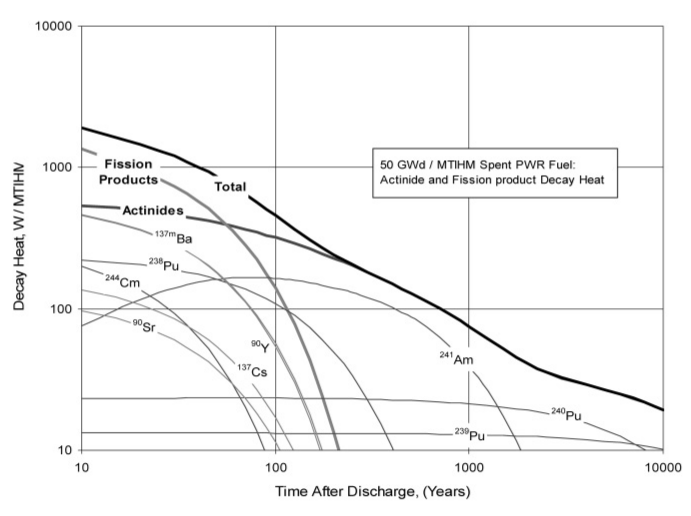
\includegraphics[scale=0.6]{./images/decay_heat.png}
	\end{center}
	\caption{Decay heat contributions in \gls{UNF} from a \gls{PWR} irradiated
		to 50 GWd/MTHM. Reproduced from Wigeland, 2006 \cite{wigeland_separations_2006}.}
	\label{fig:decay_heat}
\end{figure}


There are two major reprocessing technologies:
methods that use low-temperature chemical separation
using organic solvents (e.g. PUREX \cite{baumgaertner_purex_1976}), and
methods that use high-temperature molten salts and metals, like pyroprocessing
\cite{laidler_development_1997}. These methods separate the \gls{UNF}
into different streams, which are then sent to either a \gls{HLW} repository
(fission products) or an appropriate fuel fabrication facility (plutonium).

Different closed fuel cycles use different elemental groups for recycled
fuel fabrication. For example, the PUREX process is used in La Hague in France
\cite{schneider_spent_2008}, THORP in the U.K \cite{riley_technology_1998},
Mayak in Russia, and Rokkasho in Japan to separated plutonium and uranium
\cite{birkett_recent_2005}. The plutonium is mixed with either depleted
uranium (tails) or reprocessed uranium to produce \gls{MOX}.

Closed fuel cycles
generally involve fast-spectrum reactors to control TRU inventory.
A fast-spectrum reactor can be designed to either burn (reduce TRU),
breed (produce more TRU), or break-even (maintain TRU amount).
Selection of the fast-spectrum reactor design depends on the
goal of the deploying institution.

In this work, I only transition into fuel cycles with
continuous recycle of U/Pu or U/TRU with U fuel in fast critical reactors
(Evaluation Group 23 or 24 from the Evaluation and Screening study\cite{wigeland_nuclear_2014}).

\subsection{Fuel Cycle Transition Scenarios}
Fuel cycle transition scenarios, in this work, are when
once-through fuel cycles transition to closed fuel
cycles through the progressive replacement of previous technology
(e.g. \gls{LWR}) with an advanced technology (e.g. reprocessing
and fast-spectrum reactors). Analysis of transition scenarios requires
deliberate tracking of materials and facilities in order
to accurately calculate the resources necessary for a
successful transition.

The timescale and feasibility of a transition scenario
varies by nation, depending on the nation's nuclear energy demand
growth, fuel cycle strategies, and initial conditions.
In this work, I only consider the material feasibility of the
transition scenario. Economic and political feasibility analyses
are out of the scope of this work. A fuel cycle is is considered
materially feasible if all the deployed reactors receive fuel
in time.

The fuel demand is determined by two factors - nuclear energy demand
growth and the nation's fuel cycle strategy.
The nuclear energy demand growth determines the construction
and operation
schedule of new reactors, thus the expected fuel demand.
Fuel cycle strategies determine the isotopic
requirement of the fuel cycle transition scenario. For example,
if the transition drives toward a U-Pu \gls{MOX} fuel cycle,
plutonium inventory dominates the timescale and feasibility of transition.

Once the expected fuel demand is calculated,
the initial condition - current fissile material inventory
and reactors (and their remaining lifetimes) - determines
the material feasibility and timescale of a transition scenario.
If a transition scenario is infeasible (i.e. fissile source is lacking),
the transition can be `loosened', by delaying deployment
of advanced reactors. The energy demand is instead met by additional
deployment of previous reactor technology (e.g. \glspl{LWR}),
thereby increasing transition timescale but reducing the
intensity of fissile material demand.

Determining material feasibility of a \gls{NFC} transition scenario
requires dynamic tracking of material flows from multiple facilities,
as well as modeling of complex systems. This work
determines material feasibility by calculating
the material inventory of real-world \gls{NFC} transition scenarios.


\section{Objectives}

This thesis demonstrates and extends the real-world \gls{NFC} transition
scenario modeling capabilities in Cyclus. The goal is to
develop tools that leverage Cyclus' modularity to
add capabilities required for modeling real-world
fuel cycle transition scenarios, and demonstrate Cyclus'
capabilities by using the developed tools to perform
\gls{NFC} transition scenarios relevant to France and the United
States.

\section{Methods}
This thesis accomplishes the objective in three steps. 
First, a benchmark showed good agreement with other
fuel cycle simulation tools. \footnote{These results have been
submitted for publication in Annals of Nuclear Energy.}
Second, I identified and developed the tools and methods necessary
for modeling and simulating real-world transition scenarios.
Finally, I constructed and ran fuel cycle transition scenarios
relevant to France and the United States.

A previous study by Feng et al. \cite{feng_standardized_2016} validates existing 
\glspl{NFCS} in a fuel cycle transition scenario, in which an \gls{LWR} fleet
transitions into an \gls{SFR} fleet with continuous reprocessing. This 
study compares four well-known \glspl{NFCS}
DYMOND \cite{yacout_modeling_2005},
VISION \cite{jacobson_verifiable_2010},
ORION \cite{gregg_analysis_2012}, and
MARKAL \cite{shay_epa_2006}. The results from each code were
compared to a set of `model solutions' that were generated
from a spreadsheet for various metrics (e.g. fuel loading
in reactor, \gls{UNF} inventory). I reproduced the transition
scenario in Cyclus, and compare the Cyclus results with those
from the `model solutions'.

In order to model real-world transition into an advanced
fuel cycle, I developed two major tools. First, I developed \texttt{write\_input.py}
that automates extraction from the curated \gls{IAEA} \gls{PRIS} database
\cite{iaea_nuclear_2018}. The database lists each nuclear reactor's
country, name, type, net capacity (\gls{MWe}), status, operator, construction
date, first criticality date, first grid date, commercial date, and shutdown
date (if applicable). \texttt{write\_input.py} extracts the information from this file
to generate a Cyclus compatible input file, which lists the individual
reactor units as agents. Second, I developed a module that models \glspl{MSR}
in Cyclus using a database generated from a high-fidelity \gls{MSR} depletion calculation.
The database is an output of Saltproc [??? Cite saltproc], a python
module that drives
SERPENT 2 \cite{leppanen_serpentcontinuous-energy_2013} to model online reprocessing in an \gls{MSR}.
The database contains the historic compositions of each stream in and out of the reactor,
composition history inside the reactor, and $k_{eff}$ values. The developed tool then
reads the database to mimic \gls{MSR} behavior by requesting and offering
feed and waste material to the Cyclus framework. The database is in HDF5
format, a hierarchical data format designed to store and organize
large amounts of data \cite{the_hdf_group_hierarchical_1997}.

Finally I constructed the fuel cycle transition scenario for France and the United States.
I made different assumptions for the two scenarios to account for each nation's different goals,
initial conditions (i.e. currently existing fleet, \gls{UNF} inventory), and their potential reactor
technology. I used the \texttt{write\_input.py} to construct the initial Cyclus input file,
followed by iterations to account for new reactor deployment. The workflow driving analyses is shown in diagram \ref{diag:workflow}.


\begin{figure}
        \centering
\begin{tikzpicture}[node distance=1.5cm]
\node (database) [object] {Database (\texttt{.csv})};
\node (script) [process, below of=database] {Input Generation Script (\texttt{write\_input.py})};
\node (input) [object, below of=script] {\Cyclus Input File (\texttt{.xml})};
\node (cyclus) [process, below of=input]{\Cyclus};
\node (output) [object, below of=cyclus]{\texttt{Output File (\texttt{.Sqlite})}};
\node (script2) [process, below of=output]{Analysis Script (\texttt{analysis.py})};

\draw [arrow] (database) -- (script); 
\draw [arrow] (script) -- (input); 
\draw [arrow] (input) -- (cyclus);
\draw [arrow] (cyclus) -- (output);
\draw [arrow] (output) -- (script2);
\end{tikzpicture}
\caption{Green circles and blue boxes represent files and software 
processes, respectively, in the computational workflow.}
\label{diag:workflow}
\end{figure}


The structure of this thesis is as follows. In chapter 2, I review other fuel cycle simulation
tools and their gaps, and explain the unique capability Cyclus
has for transition scenario simulation.
Chapter 3 explains the design and
the development of capabilities needed for \gls{NFC} transition simulation.
Chapter 4 shows the results from the benchmark study, in which Cyclus results are compared
to results from other fuel cycle simulation tools.
Chapter 5 and 6 show the results from the France and United States fuel cycle
transition scenario.
